\subsection{Post Module}
\par{The post model will be a service used to post messages to the forum. The messages will be in the form of either posts and comments.}
\subsubsection{Requirements}
\subsubsection*{Functional}
\begin{itemize}
\item Handle the posting and accessing of forum content as well as structuring forum threads in an orderly manner.
\item Three types of posts can be made. The creation of a thread (level-zero post), the response to a post and the creation of a bounty post. 
\end{itemize}

\subsection*{Types of posts}
\begin{itemize}
\item {Level-zero post: The first post for a specified topic is termed a level-zero post. A topic will only have one level-zero post which can be seen as a the root in a hierarchy of related posts}
\item {Child-post: Responses to posts are termed child-posts. Child posts become parent posts to other posts when responses are made to that child post.}
\item {Sibling-Post: Posts at the same level within the same topic are termed sibling posts.}
\item {Bounty-post: Users are able to make posts in the form of questions with an attached reward to be awarded to the person who gives a correct answer to this question. We call such a post a bounty-post. This feature forms part of the gamification module and will be further more discussed in the Gamification module.}
\end{itemize}

\subsubsection{Use cases}
\subsubsection*{Create Post}
\par{This will be a functionality which will allow users to create new posts for the course module they belong to. If they are adding on to an already existing post then it will fall under that post. The posts structure will follow a tree structure. Upon creating a post, tags will also be created that accompany that post.}
\subsubsection*{Edit Post}
\par{This will be a service for users with higher privileges. It will allow them to edit various posts. The main edits will be on tags of a post.}
\subsubsection*{Remove Post}
\par{This will be a service for users with higher privileges. It will allow them to remove various posts, meaning that they will no longer be visible to other users. When a post is removed, all the posts and comments that accompany and fall under it will also be removed.}
\subsubsection{Domain Model}
\begin{itemize}
\item A new post will be on level 0, making its heading the name of the thread.
\item The level of a new post, under another post, will be an increment of the post that it falls under.
\item A post cannot be created by a user who does not belong to the module. 
\end{itemize}
\begin{figure}[h!]
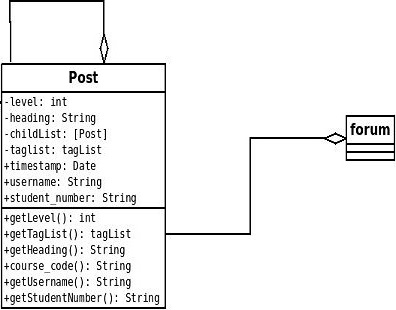
\includegraphics{Diagrams/posts_domain_model.jpeg}
\caption{Domain model representing the message model}
\label{fig:mesg}
\end{figure}